\documentclass[
]{article}

\usepackage{graphicx}

\author{Weihao Jiang}
\date{Dec. 2020}

\begin{document}

\title{AVORHOD}
\maketitle

\begin{abstract}

AVORHOD is a computer program that provides Analysis and Visualization
of Online Ride-Hailing Order Data. By processing, classifying and
visualising the start, end, time and price information of each order in
Online Ride-Hailing's order data, AVORHOD helps data analysis experts to
better find the relationship between demand and time distribution and
helps Online Ride-Hailing's algorithm designers to further optimise The
AVORHOD program helps data analysis experts to better find the
relationship between demand and time, and helps the algorithm designers
at Online Ride-Hailing to further optimise their algorithms.

The program solves large-scale data processing problems that are
difficult to handle with conventional Excel and Python scripts through
sequential execution of queues based on SQLite data structures, and
provides a better system of visualisation and analysis tools.

\end{abstract}

\section{Introduction}

AVORHOD provides visual data analysis through a combination of two
designs.

The first is a data manipulation daemon thread. A sequential execution
queue inside this daemon thread enables efficient finding of what is
needed between large amounts of data and prevents data corruption caused
by concurrent operations.

The second is a chart generation system. With the help of the
diagramming module provided by Qt, this application is able to provide
as many analytical relationships and diagrams as possible and present
them quickly in a variety of, customisable ways.


\section{Implementation details}

\subsection{Data storage}

This program uses internally a data storage based on SQLite, a
file-based micro-database that not only allows for efficient indexing of
traditional databases, ready to be used in a single read, but also
offers better possibilities for later cached use.

There are two tables in the database: the data section and the grid
information section. The reason why the grid information is also stored
in the database is to make queries to the database more atomic and to
ensure that low blocking is maintained even after the grid is increased.

All data operations are performed by a daemon thread uniquely connected
to the database. The daemon thread implements transactional queue
processing via a sequential execution queue, which guarantees sequential
reads and writes and prevents data file corruption from concurrent read
and write processes that may arise at high frequencies in the program.

All interactions with the daemon are asynchronous through the
signal-slot mechanism provided by Qt. From read operations that can
block for up to half a minute, to query operations that block for less
than a second, the daemon is passed through in the form of signals and
grasses to minimise blocking to the master process. The data is read and
written using the SQL language as middleware, which also gives the
program relatively good flexibility and scalability.

Although there is a confirmation key on the read screen, in order for
the program to read in quickly and not take up any more time, the
reading starts as soon as the user has selected the location of the data
file. Although the requirements imply that data that is not of interest
to the user should be removed, the full data store is retained for the
integrity of the data index and only the content that is not of interest
to the user is removed during interaction with the user. In fact, this
avoids the inefficiency of having C++ do the in-memory splicing of
strings (which usually means countless copies everywhere), and instead
makes the selection via the interpreter of the SQL script. Within the
cache of such an interpreter, it is usually domain-definite and fast.

\subsection{Visual analysis}

Given that we don't know what content is related to each other - it
makes little sense to look at their graphs if we know the connections,
it's like shooting an arrow before drawing a target.

The program therefore provides a set of variable graphing tools similar
to those in TI-84. A unified graphical interface allows the user to use
the program to generate any number of images for univariate and
time-varying variables, including bar, line and pie charts.

The interface also offers a high degree of customisation. This allows
the user to choose whether to smooth the curve, present it in a
cumulative or distributed form, count or sum the internal factors (e.g.
if the user wishes to count the accumulation of costs over time, it is
often desirable to sum the internal factors to calculate the total
price, whereas when counting the distribution of costs, summing would
not be mathematically meaningful).

The generation of images is also dependent on a data daemon thread and
is implemented asynchronously as it involves querying the data so that
it does not block the main process. However, user requests to generate
charts are supported for concurrent operations, with signals triggered
in the main process.

\section{Results and discussion}

The visual analysis of some typical data gives some typical information,
such as the user distribution showing a change in a day-by-day cycle,
and the fact that there is significantly less traffic in the edge plots
than in the central plots.

\begin{center}
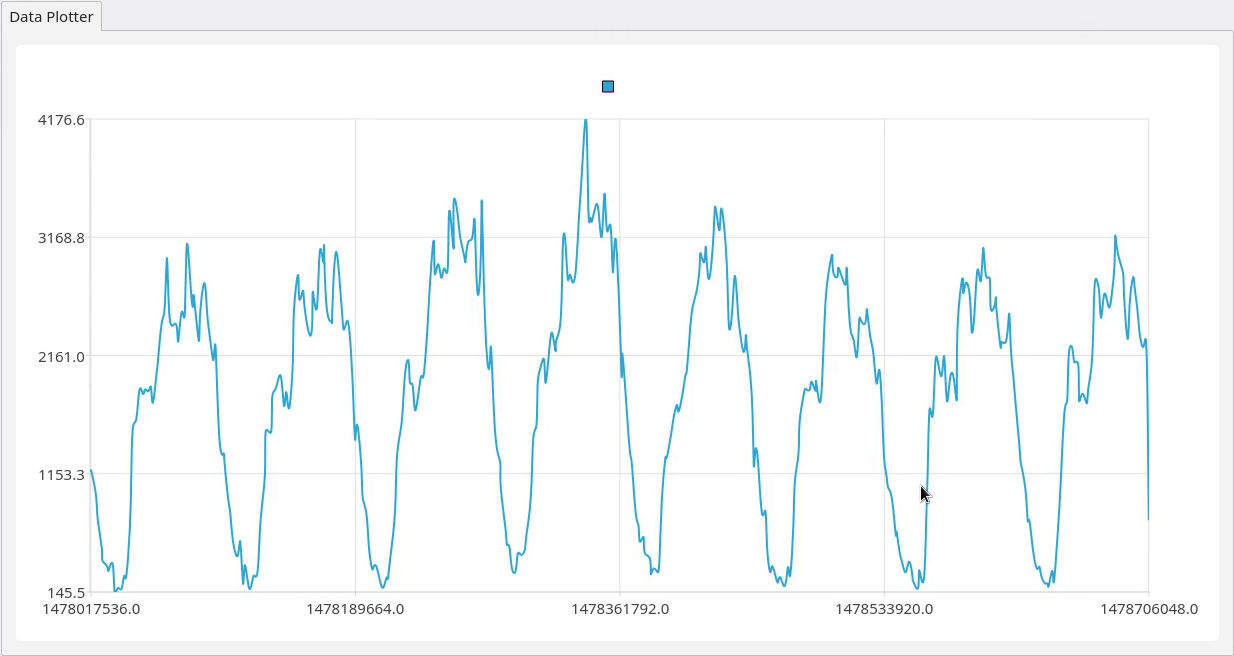
\includegraphics[width=0.7\linewidth]{./p1.png}

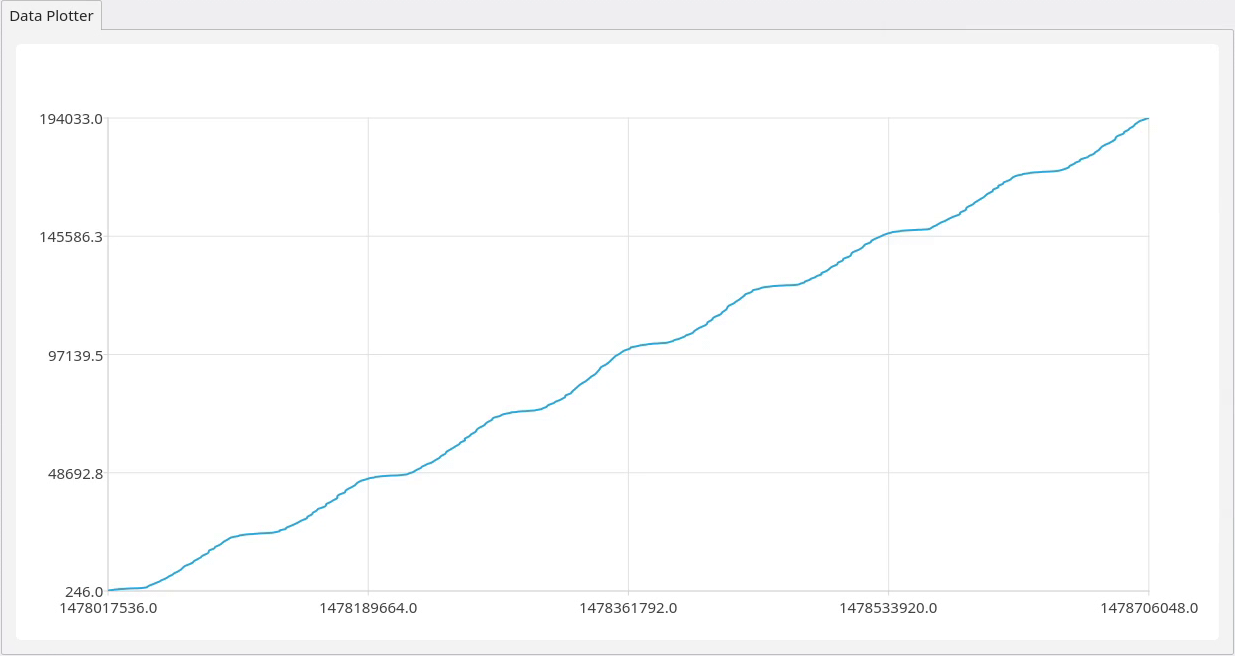
\includegraphics[width=0.7\linewidth]{./p2.png}
\end{center}


The performance of the program. It only takes about thirty seconds to
read the approximately 400MB of data provided. This result would
probably be better if we did not need to display the progress of the
read in parallel.

Our program does not include an index because the entire query is short,
less than half a second, but adding an index would double the disk space
used by the program. For a graph of 3 million data, i.e. the entire data
table, the time from start to image load is less than 1 second.

Of course, the program does not block during the image load. That is, if
you are fast enough, you can draw a second image while the image is
loading.

\end{document}
